\subsection[Návrh replikačního řešení]{Návrh replikačního řešení}
      \label{kNavrh}

      Po provedení rešerše a zohlednění všech podmínek, požadavků a možností katedry, byl sestaven návrh kompletního databázového řešení založeného na procesu replikace. Z databázových serverů, diskutovaných v kapitole \odkazKapitola{kPouziteProstredky}, byl vybrán server PostgreSQL hned z několika důvodů. Jedná se o plnohodnotný databázový systém dostupný zdarma se všemi nástroji, je široce používaný v oblasti geoinformačních technologií, je multiplatfomní a od verze ArcGIS 9.3 plně podporováný produkty ArcGIS. Návrh počítá s použitím ArcSDE pro propojení databáze s ArcGIS produkty. Při výběru jednotlivých verzí je nutné zajistit kompatibilitu verzí jednotlivých software, viz kapitola \ref{kArcSDE} a poté ArcSDE nainstalovat na servery v clusteru.

Byl navržen replikační cluster s nejméně třemi servery z důvodů, které již byly diskutovány v kapitole \odkazKapitola{kReplikace}. Celý cluster poběží na stejné platformě a proto bude možno použít streaming replikaci se všemi výhodami a nevýhodami zmíněnými v kapitole \odkazKapitola{kStreamingTeorie}. Byla zvolena jednosměrná master-slave replikace, cluster tedy bude obsahovat jeden master a dva (popř. více) slave serverů. Aby nedošlo ke ztrátě dat v případě, že by master server spadl dřív, než se data zkopírují na slave server, pro první slave (slave1) byla zvolena varianta synchronní replikace. Je vhodné, aby servery běžely v~lokální síti z důvodu rychlosti a spolehlivosti spojení mezi master a slave serverem. 

      \begin{figure}[H]
        \label{oNavrhKatedra}
        \centering
        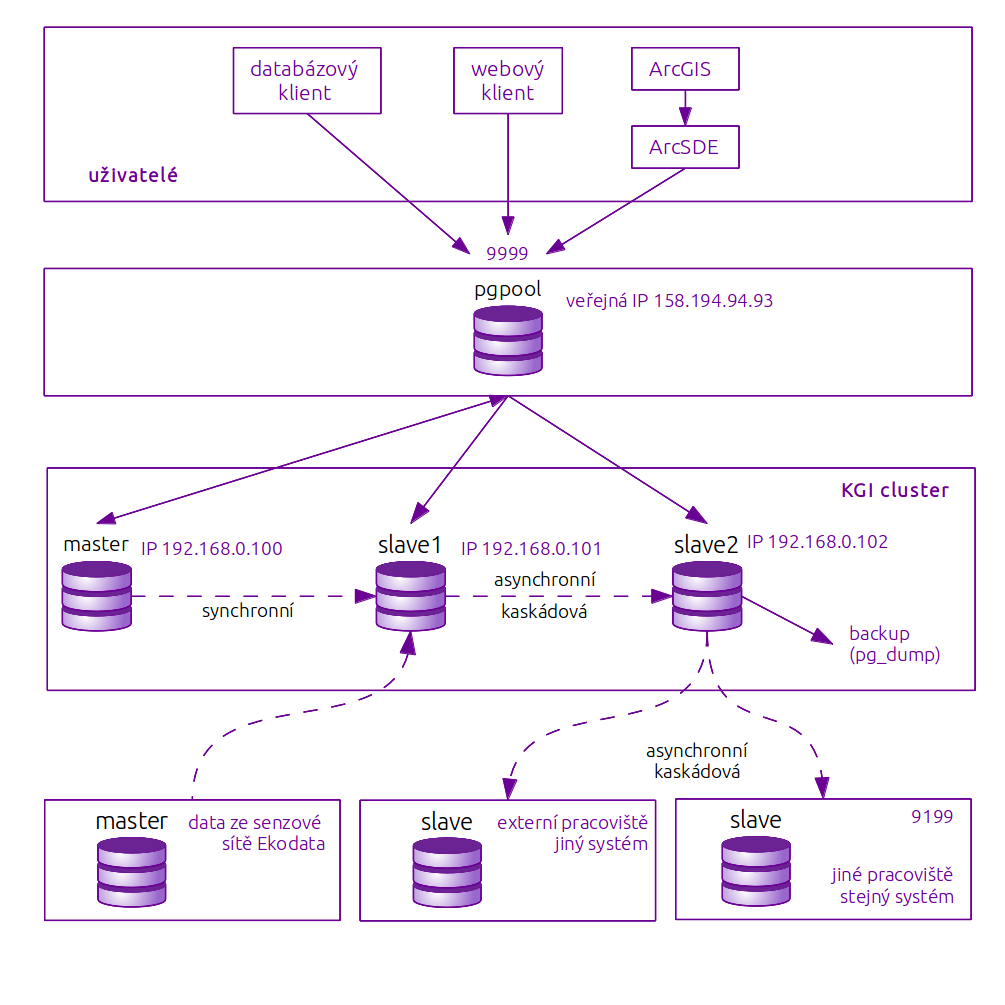
\includegraphics[scale=1]{../../../grafy/obr/schema_navrhKatedra.png}
        \caption {Návrh replikačního řešení}
      \end{figure}

      Druhý server (\texttt{slave2}) bude replikovat asynchronně a zároveň, aby nedocházelo k~přetížení master serveru, bude replikace probíhat ze \texttt{slave1} na \texttt{slave2}, tedy kaskádově. Tím bude řešení zároveň přípraveno na výpadek master serveru, protože v případě master vypadne, \texttt{slave1} bude povýšen na master a \texttt{slave2} bude ihned moci replikovat. Ze \texttt{slave2} lze dále tvořit pravidelnou, například denní nebo týdenní, zálohu pomocí ulitily \texttt{pg\_dump}, která je více popsána v kapitole \odkazKapitola{kPriprava}. Záloha pomocí \texttt{pg\_dump} tak nebude zatěžovat master server a sama o sobě bude probíhat rychleji, než by tomu bylo na master serveru, který je již tak velmi vytížen dalšími procesy.

Uživatelé se budou připojovat skrze pgpool, jehož výhody a možnosti byly popsány v kapitole \odkazKapitola{kpgpool}. pgpool se bude tvářit jako jediný databázový server, ke kterému se klienti přihlásí bez ohledu na typ jejich dotazu a on sám pak rozhodne, ke kterému ze serverů klienta přihlásí. Tím bude mít zároveň možnost rozložit zátěž na dostupné uzly v clusteru. Pro ještě větší efektivitu provozu databáze bude pgpool uchovávat databázová spojení a při novém dotazu využije stávajícího spojení, místo aby vytvářel spojení nové. 

Vzhledem k tomu, že klienti budou k databázovému serveru přistupovat skrze pgpool, není potřeba aby jednotlivé uzly v clusteru měly veřejnou IP adresu. Plně dostačuje, že servery poběží na lokální síti a pouze pgpool bude na serveru s veřejnou IP, čímž se zajistí, že data budou přístupná z internetu. 

Návrh počítá také s externími pracovišti, která budou často číst z databáze a~budou mít zájem o zrychlení přístupu k datům tím, že se slave server přesune na jejich pracoviště. Typ replikace se zvolí podle jejich operačního systému a jeho architektury. Pokud se bude jednat o shodný systém, jaký bude použit ve výše popsaném clusteru, pak bude možno použít asynchronní streaming replikaci, naopak pokud se bude bude jednat o systém jiný, bude použita Slony-I replikace. 

